Grundlegend für Streuexperimente ist der Wirkungsquerschnitt $\sigma$.
Der Wirkungsquerschnitt beschreibt die Wechselwirkungswahrscheinlichkeit einer Projektils mit einem bestimmten Target.
Dabei hat $\sigma$ die Dimension einer Fläche und beschreibt anschaulich eine 'Wechselwirkungsfläche' des jeweiligen Atoms im Target.
Je größer die Fläche, desto wahrscheinlicher die Streuung.
\begin{figure}[h!]
  \centering
  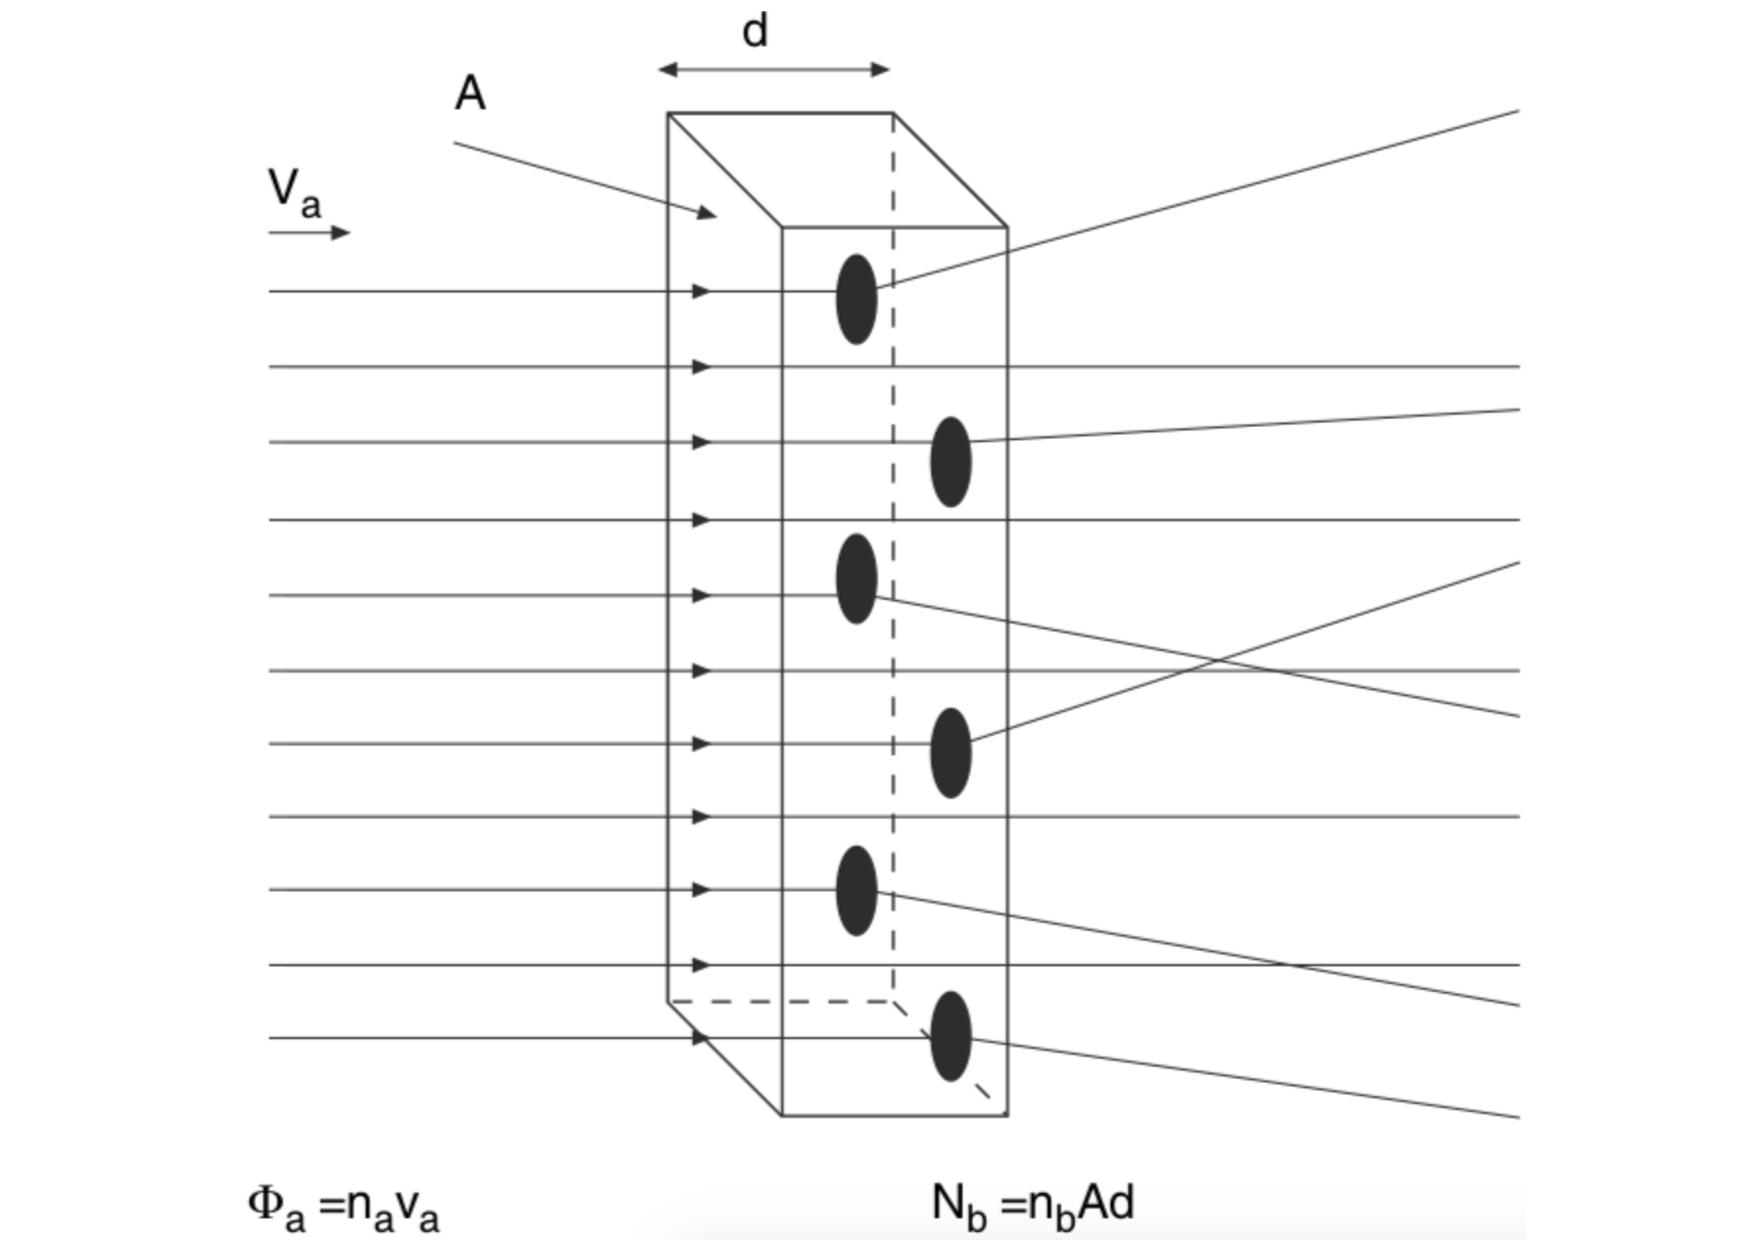
\includegraphics[width=0.6\textwidth]{images/wq.pdf}
  \caption{Anschauliche Beschreibung des Wirkungsquerschnitts $\sigma$ \cite{povh}}
  \label{fig:wq}
\end{figure}

%Theorie
%Wirkungsquerschnitt
%- Was ist das allgemein?
%
%Bethe-Bloch
%- Absorption von geladenen schweren Teilchen
%- Plot?
%- Formel
%- Näherungen
%
%Differenzieller Wirkungsquerschnitt
%- Herleitung?
%- Rutherfordstreuung herleiten
%- Formel
%- Näherungen
